\documentclass[fleqn,12pt,a4paper]{olplainarticle}
% Use option lineno for line numbers 

\usepackage{hyperref}
\usepackage{graphicx}
\usepackage{vhistory}
\usepackage{setspace}
\usepackage{etoolbox}

\usepackage{array}

\pdfpageheight=\paperheight
\pdfpagewidth=\paperwidth
\setlength\oddsidemargin{\dimexpr(\paperwidth-\textwidth)/2 - 1in\relax}
\setlength\evensidemargin{\oddsidemargin}

\title{DUNE Timing System (DTS) Safety Engineering Design Review (SEDR) Documentation for GPS Interface Board (GIB)}

\author[1]{D. Cussans}
\author[2]{J. Sensenig}
\author[1]{S. Trilov}
\affil[1]{H.H. Wills Physics Laboratory, Bristol, UK}
\affil[2]{David Rittenhouse Laboratory, Philadelphia, USA}

\AtBeginEnvironment{tabular}{\doublespacing}

\newcolumntype{L}[1]{>{\raggedright\let\newline\\\arraybackslash\hspace{0pt}}m{#1}}
\newcolumntype{C}[1]{>{\centering\let\newline\\\arraybackslash\hspace{0pt}}m{#1}}
\newcolumntype{R}[1]{>{\raggedleft\let\newline\\\arraybackslash\hspace{0pt}}m{#1}}

\begin{document}


\keywords{DUNE,Timing System,Safety,SEDR,GIB}

\begin{abstract}
This document provides information needed for a review of the electrical safety of the DUNE Timing System(DTS) GPS Interface Board (GIB). A overview of the electrical safety of the DTS hardware is given in EDMS document \href{https://edms.cern.ch/document/3057172/1}{EDMS 3057172}\cite{ref:dts-sedr-overview} and should be read in conjunction with this document.

\textsc{document source:}\\
{\bf EDMS:} xxxxxx \\
{\bf Overleaf:}  \url{https://www.overleaf.com/read/pkbtxcsyysyt\#0d8f4a}

\end{abstract}


\flushbottom

\maketitle

% Start of the revision history table
\begin{versionhistory}
  \vhEntry{1.0}{10/Jan/25}{DGC}{created}
\end{versionhistory}

\section*{Document Approvals}

\begin{table}[tbh]
    \centering
    \begin{tabular}{p{0.6\textwidth}|R{0.35\textwidth}}
        Signatures Required   &  Signature and Date Approved\\ \hline
        Originator: D. Cussans                     &  AAAA  X/YYY/ZZ \\
        Approver: R. Sipos (DAQ Technical Lead)    &  AAAA   X/YYY/ZZ  \\
        Approver: W. Ketchum (DAQ Consortium Lead)    &  AAAA    X/YYY/ZZ  \\
        Approver: T. Shaw (DUNE Compliance Office) &  AAAA X/YYY/ZZ           \\
    \end{tabular}
    \label{tab:approvals}
\end{table}
\newpage
%\thispagestyle{empty}

\section{Introduction}

The DUNE Timing System has hardware components both above ground and below ground. At the far detector the above ground hardware will be at the SURF Ross and Yates areas and the below ground in the DAQ cabins above each far detector cryostat. At the near detector the above ground hardware will be at Fermilab in a location accessible to cables carrying synchronization information from the accelerator complex with the below ground hardware in the near detector hall.

The above ground hardware at each of the Ross and Yates areas consists of a COTS GPS disciplined oscillator with associated antenna, lightning protection etc. providing timing information to a custom GPS Interface Board (GIB). The below ground hardware in each of the far detector caverns consists of a COTS MicroTCA crate housing COTS PSUs, MCH, JSM and fan-trays along with a custom MicroTCA Inteface Board (MIB) and multiple semi-custom FPGA based AFC boards hosting custom Fibre Interface Boards (FIBs). Each far detector cavern will have two MicroTCA crates.
Figure \ref{fig:dts_fd_block_diagram} illustrates the location of DTS hardware at the far detector.

\begin{figure}[ht]
\centering
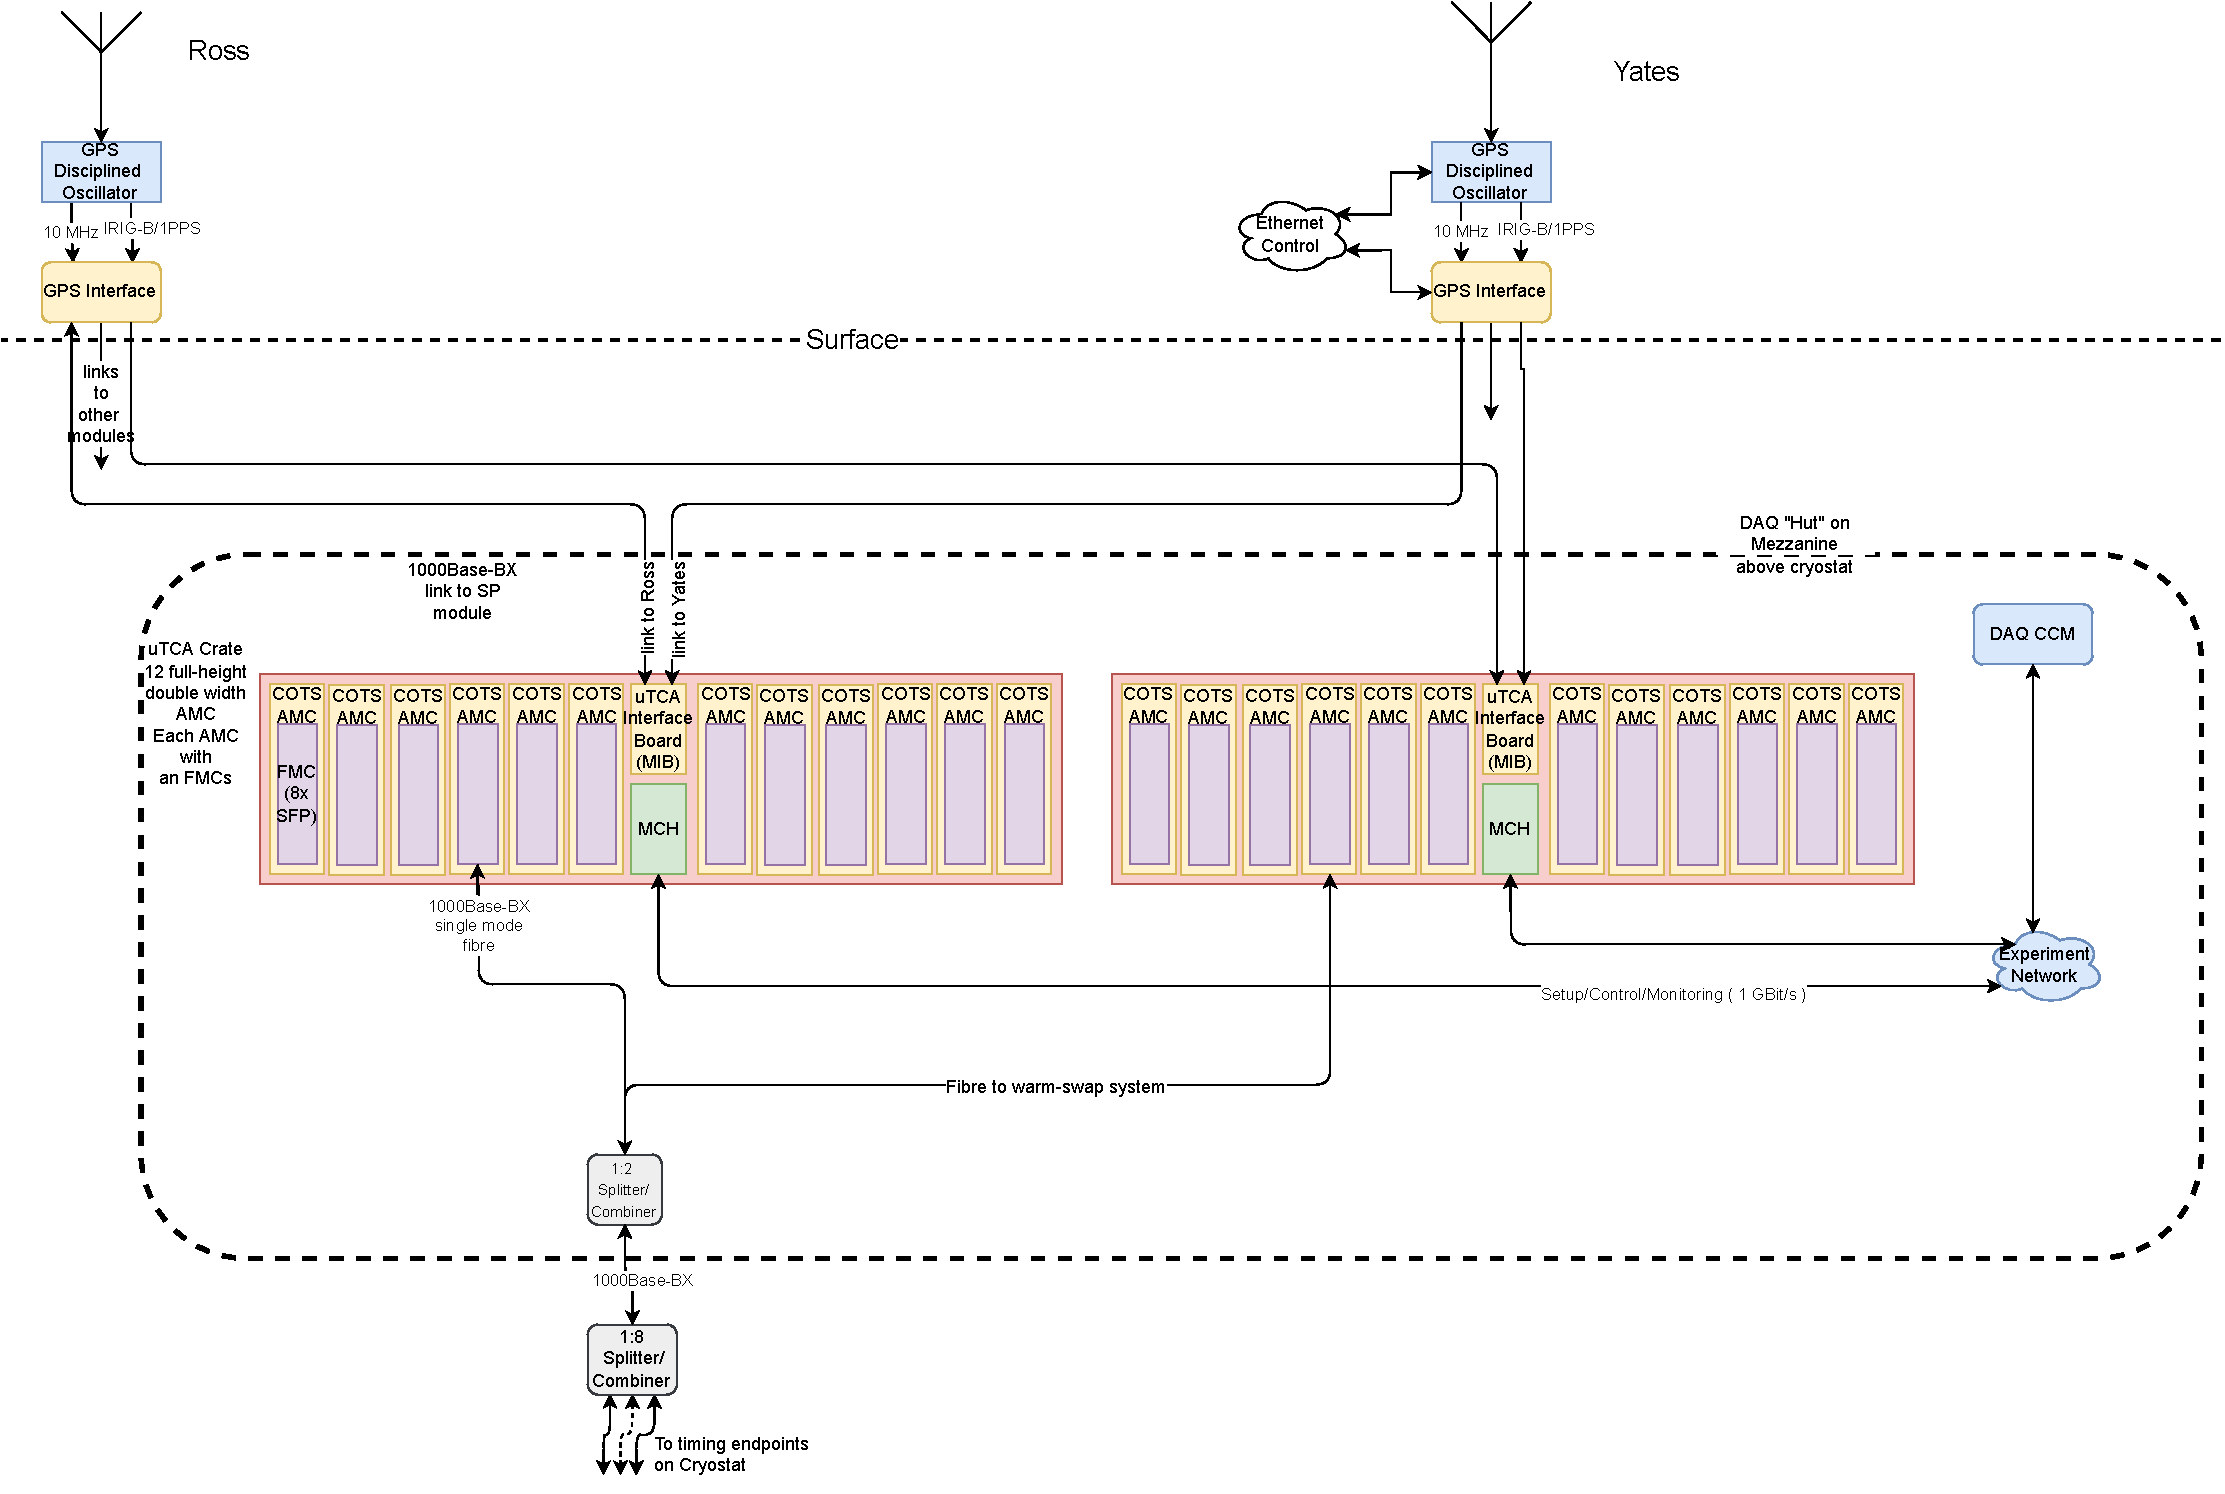
\includegraphics[width=\linewidth]{dune_timing_system_block_diagram_twepp22_1sept22_02.drawio.pdf}
\caption{Block Diagram of DUNE Far Detector Timing Hardware.}
\label{fig:dts_fd_block_diagram}
\end{figure}

\subsection{Overview of the GPS Interface Board (GIB)}

The GIB, the subject of this review, is coupled to a COTS FPGA module via a standard low pin count FMC connector\cite{ref:fmc}.
%(Enclustra \href{https://www.enclustra.com/en/products/fpga-modules/mars-ax3/}{AX3}/\href{https://www.enclustra.com/en/products/base-boards/mars-pm3/}{PM3} combination) 
and mounted in a custom 19-inch rack mounting enclosure. Power is provided at 12V from an external COTS AC-DC power supply. Figure \ref{fig:dts_gib_power_block_diagram} illustrates the powering arrangements for the GIB. In addition to over-current protection provided by a fuse, temperature control and monitoring will be provided an separate PCB housing ESP32 micro-controller implementing an  OPC/UA server\cite{ref:opc_ua}. Figure \ref{fig:dts_gibV1_photo} shows the current GIB prototype.

\begin{figure}[ht]
\centering
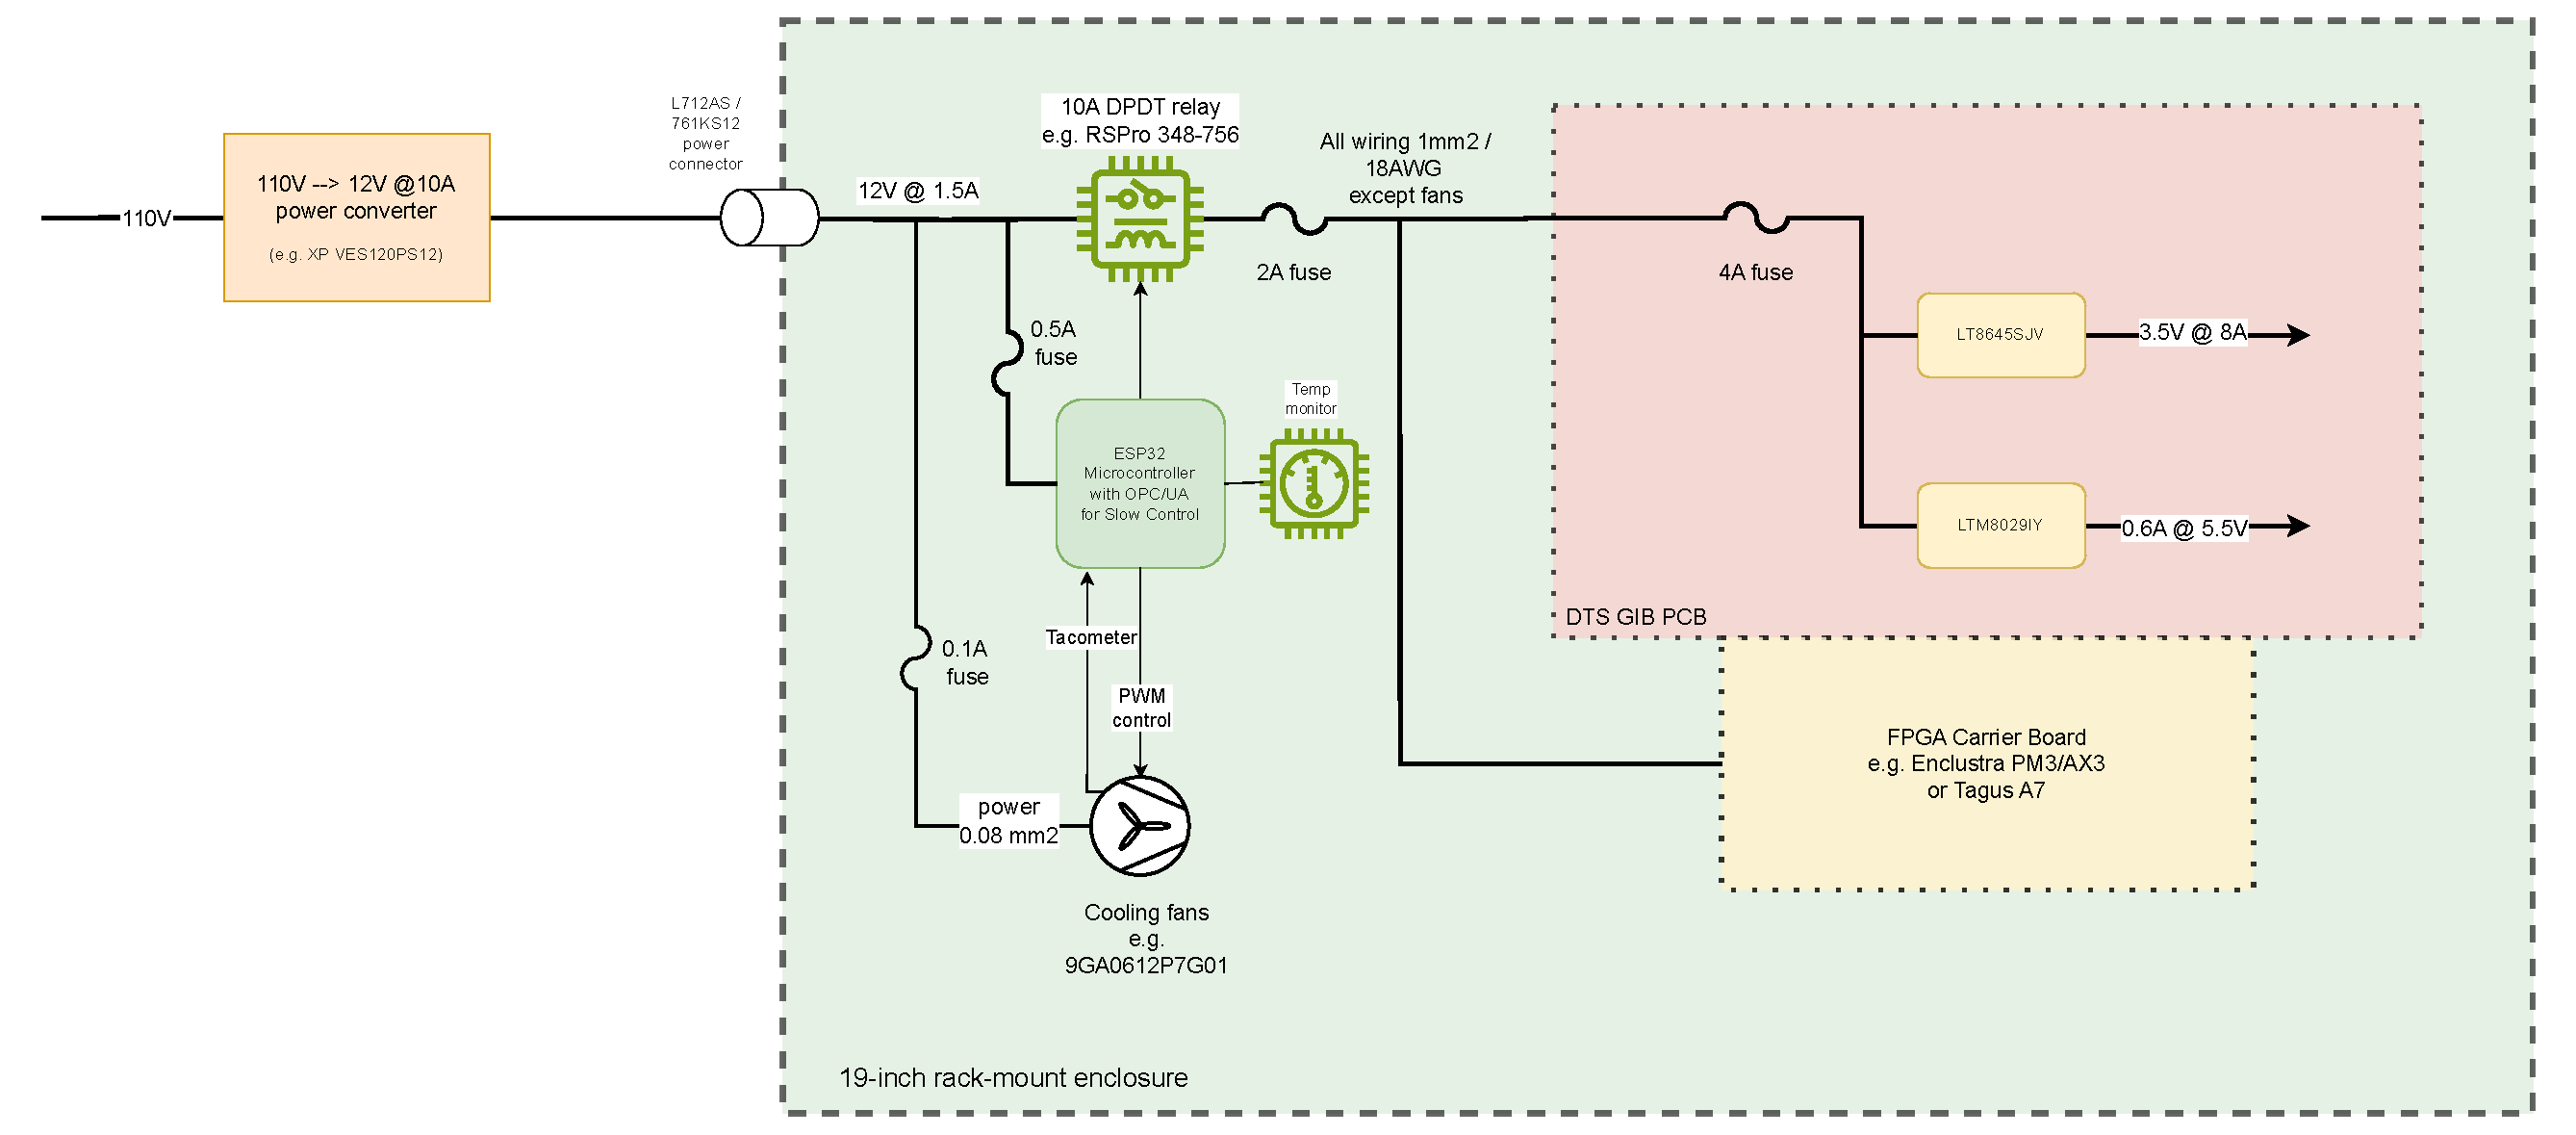
\includegraphics[width=\linewidth]{dts_gib_power_block_diagram_v3-250411.drawio.pdf}
\caption{Block diagram of powering arrangements for GIB}
\label{fig:dts_gib_power_block_diagram}
\end{figure}

\begin{figure}[ht]
\centering
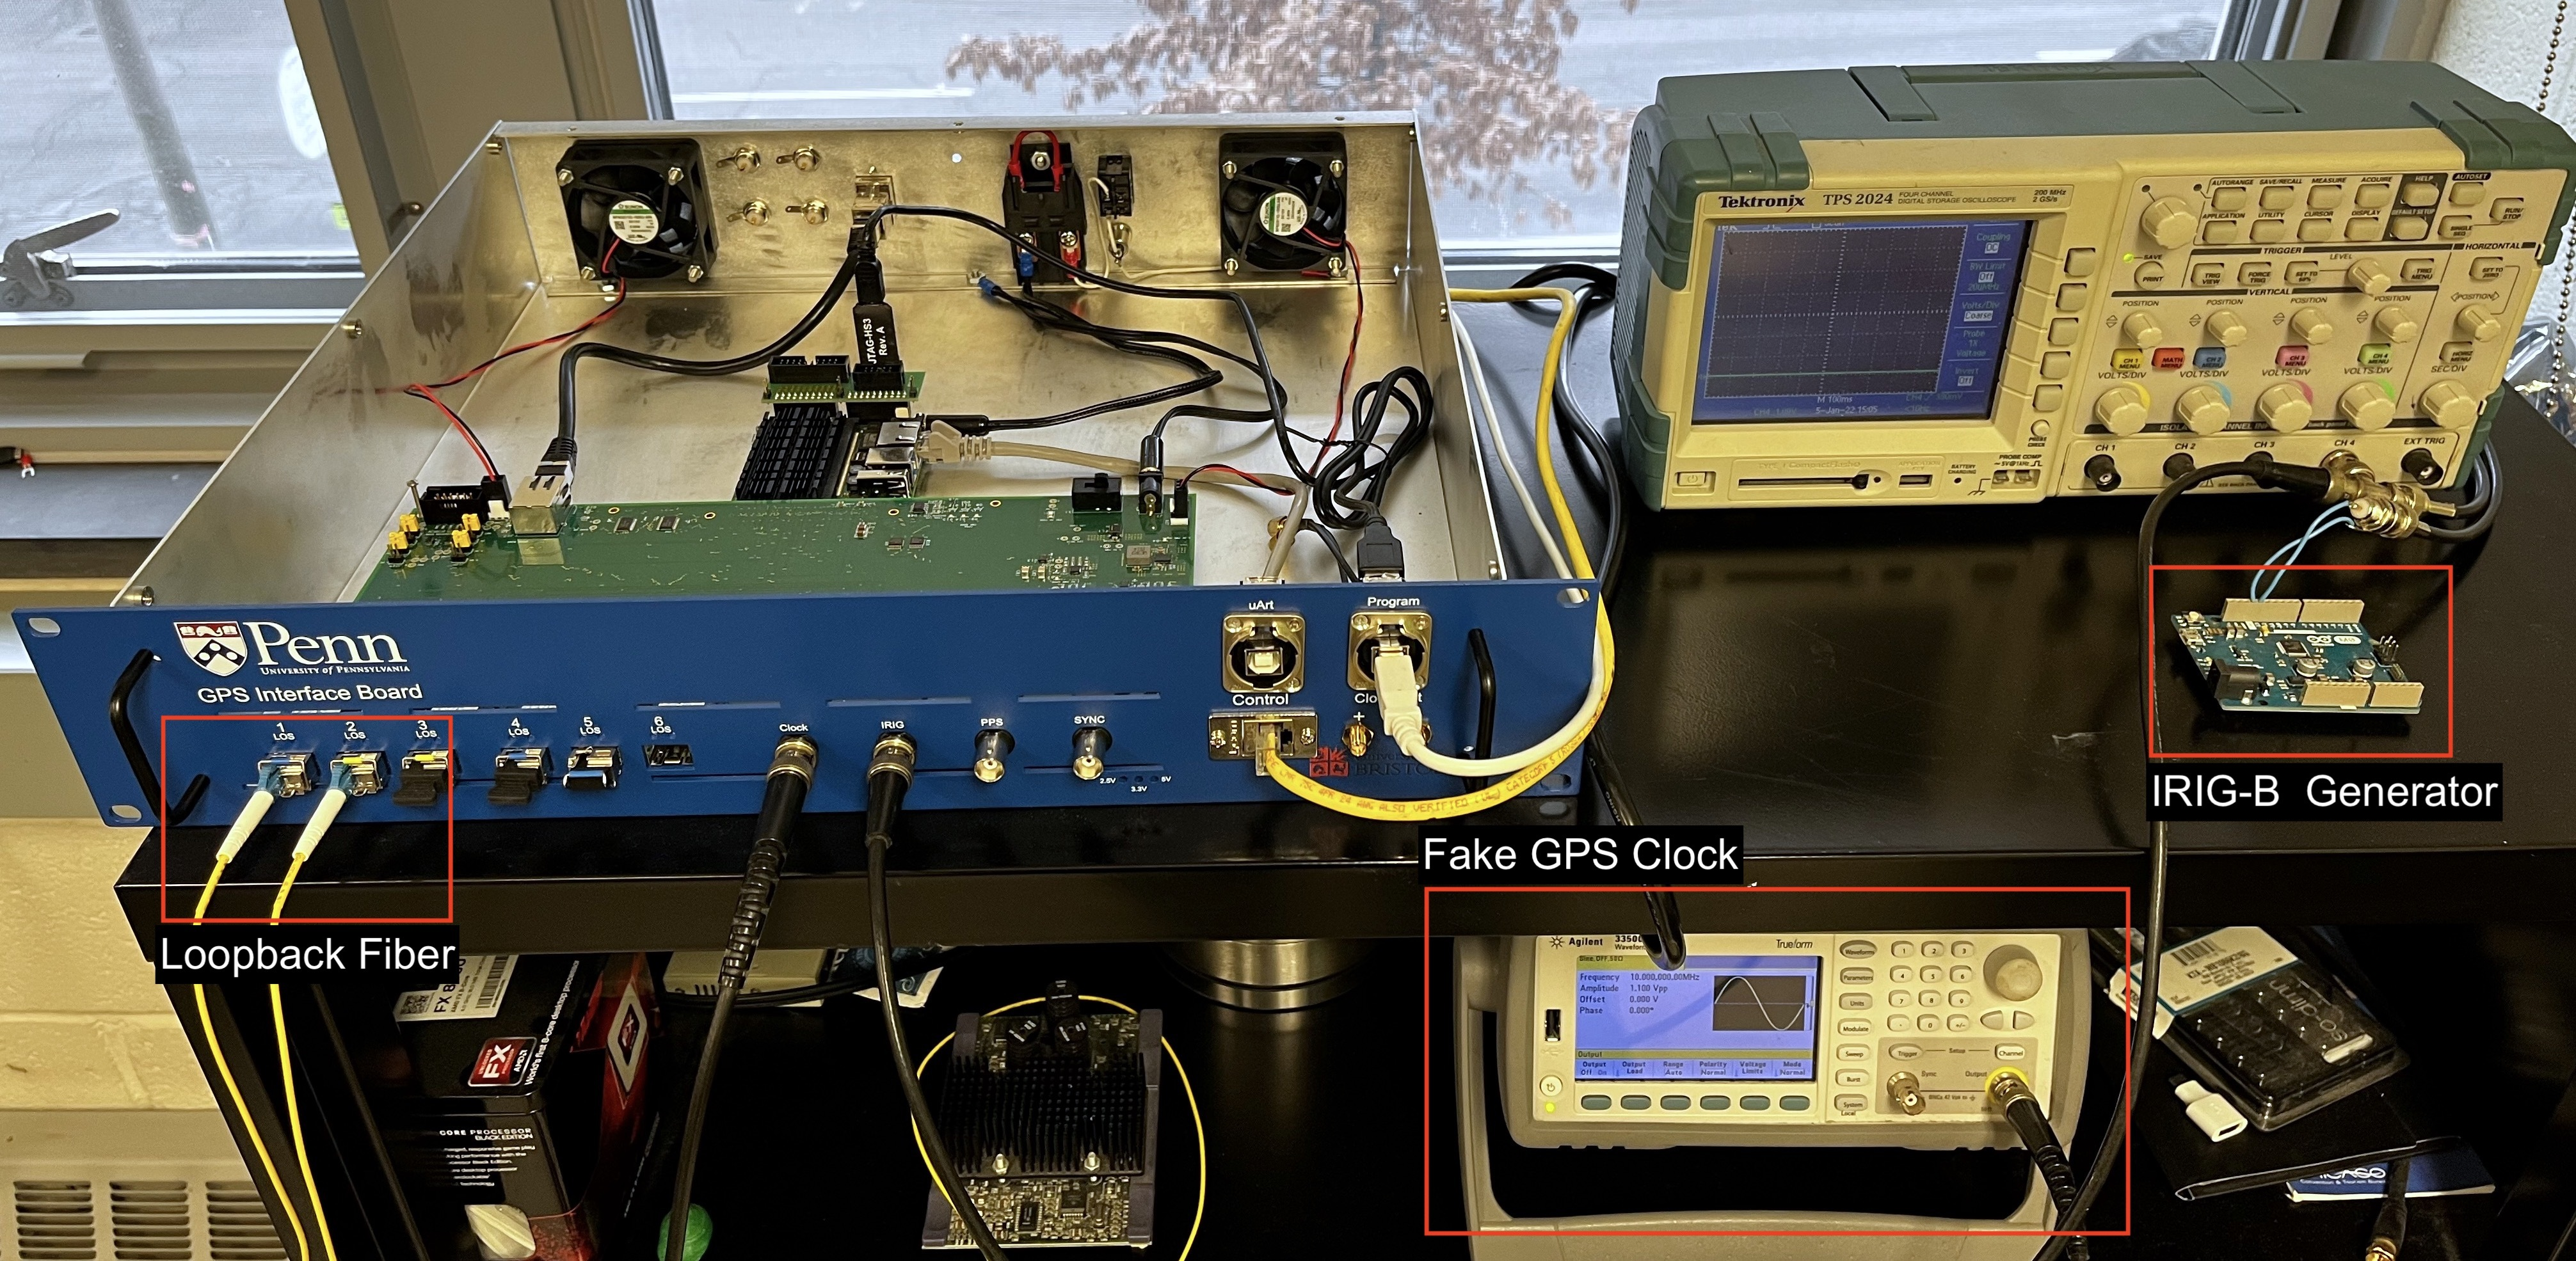
\includegraphics[width=0.85\linewidth]{gib_teststand_setup_annotated.JPG}
\caption{Photograph of current GIB prototype}
\label{fig:dts_gibV1_photo}
\end{figure}

\section{GIB Main PCB}

The GIB main PCB is powered from 12V with DC-DC converters stepping this down to 5.5V and 3.5V with linear regulators producing 5V , 3.3V and 2.5V rails.

Measurements indicate that the current drawn during operation from the 12V  by the GIB main PCB is 1.6A.

Power enters the main PCB via a \href{https://www.molex.com/en-us/products/part-detail/1724480004}{Molex 172448-0004} connector. There are two contact for 12V and two for the return current. Each contact is rated at 13A. The 12V supply current then flows through a fuse rated at 4A.

Fused 12V power is connected to a copper area of approximately 40mm x 50mm on PCB layer 5 by 12 vias each with 0.4mm finished hole size . The ``Via Current Capacity Table'' at \url{https://artist-3d.com/via-current-capacity/} indicates that in isolation each 0.4mm via can carry up to 1.5A each. The via capacity table is illustrated in \ref{fig:via-current-table}. Because the vias are clustered together the maximum current capacity will be less than twelve times the capacity of an isolated via. Using a 2/3 de-rating factor (from FNAL ESH DocDB Document 2781-v8\cite{ref:fnal-esh-design-standards}) the maximum safe current capacity is 12 x 1.5A x 2/3 = 12A - well in excess of the 4A fuse.

The current carrying capacity of the copper plane  is difficult to estimate but clearly in excess of the 4A permitted by the fuse.

The DC-DC switched mode power converters are connected to the copper area on layer 5 by at least four vias each, with a maximum current capacity of 
4 x 1.5A x 2/3 = 4A . This is marginal but believed to be acceptable even if one of the power converters fails short circuit.

\begin{figure}
    \centering
    \includegraphics[width=\linewidth]{How to Design PCB Via Current Capacity _ - Artist 3D — Mozilla Firefox 26_03_2024 17_49_05.png}
    \caption{Table listing maximum current per via}
    \label{fig:via-current-table}
\end{figure}

The main PCB is a 10 layer 2.5mm thick PCB. The stack up is shown in figures \ref{fig:gib_main_pcb_cross_section_figure} and \ref{fig:gib_main_pcb_cross_section_details}.

\begin{figure}
    \centering
    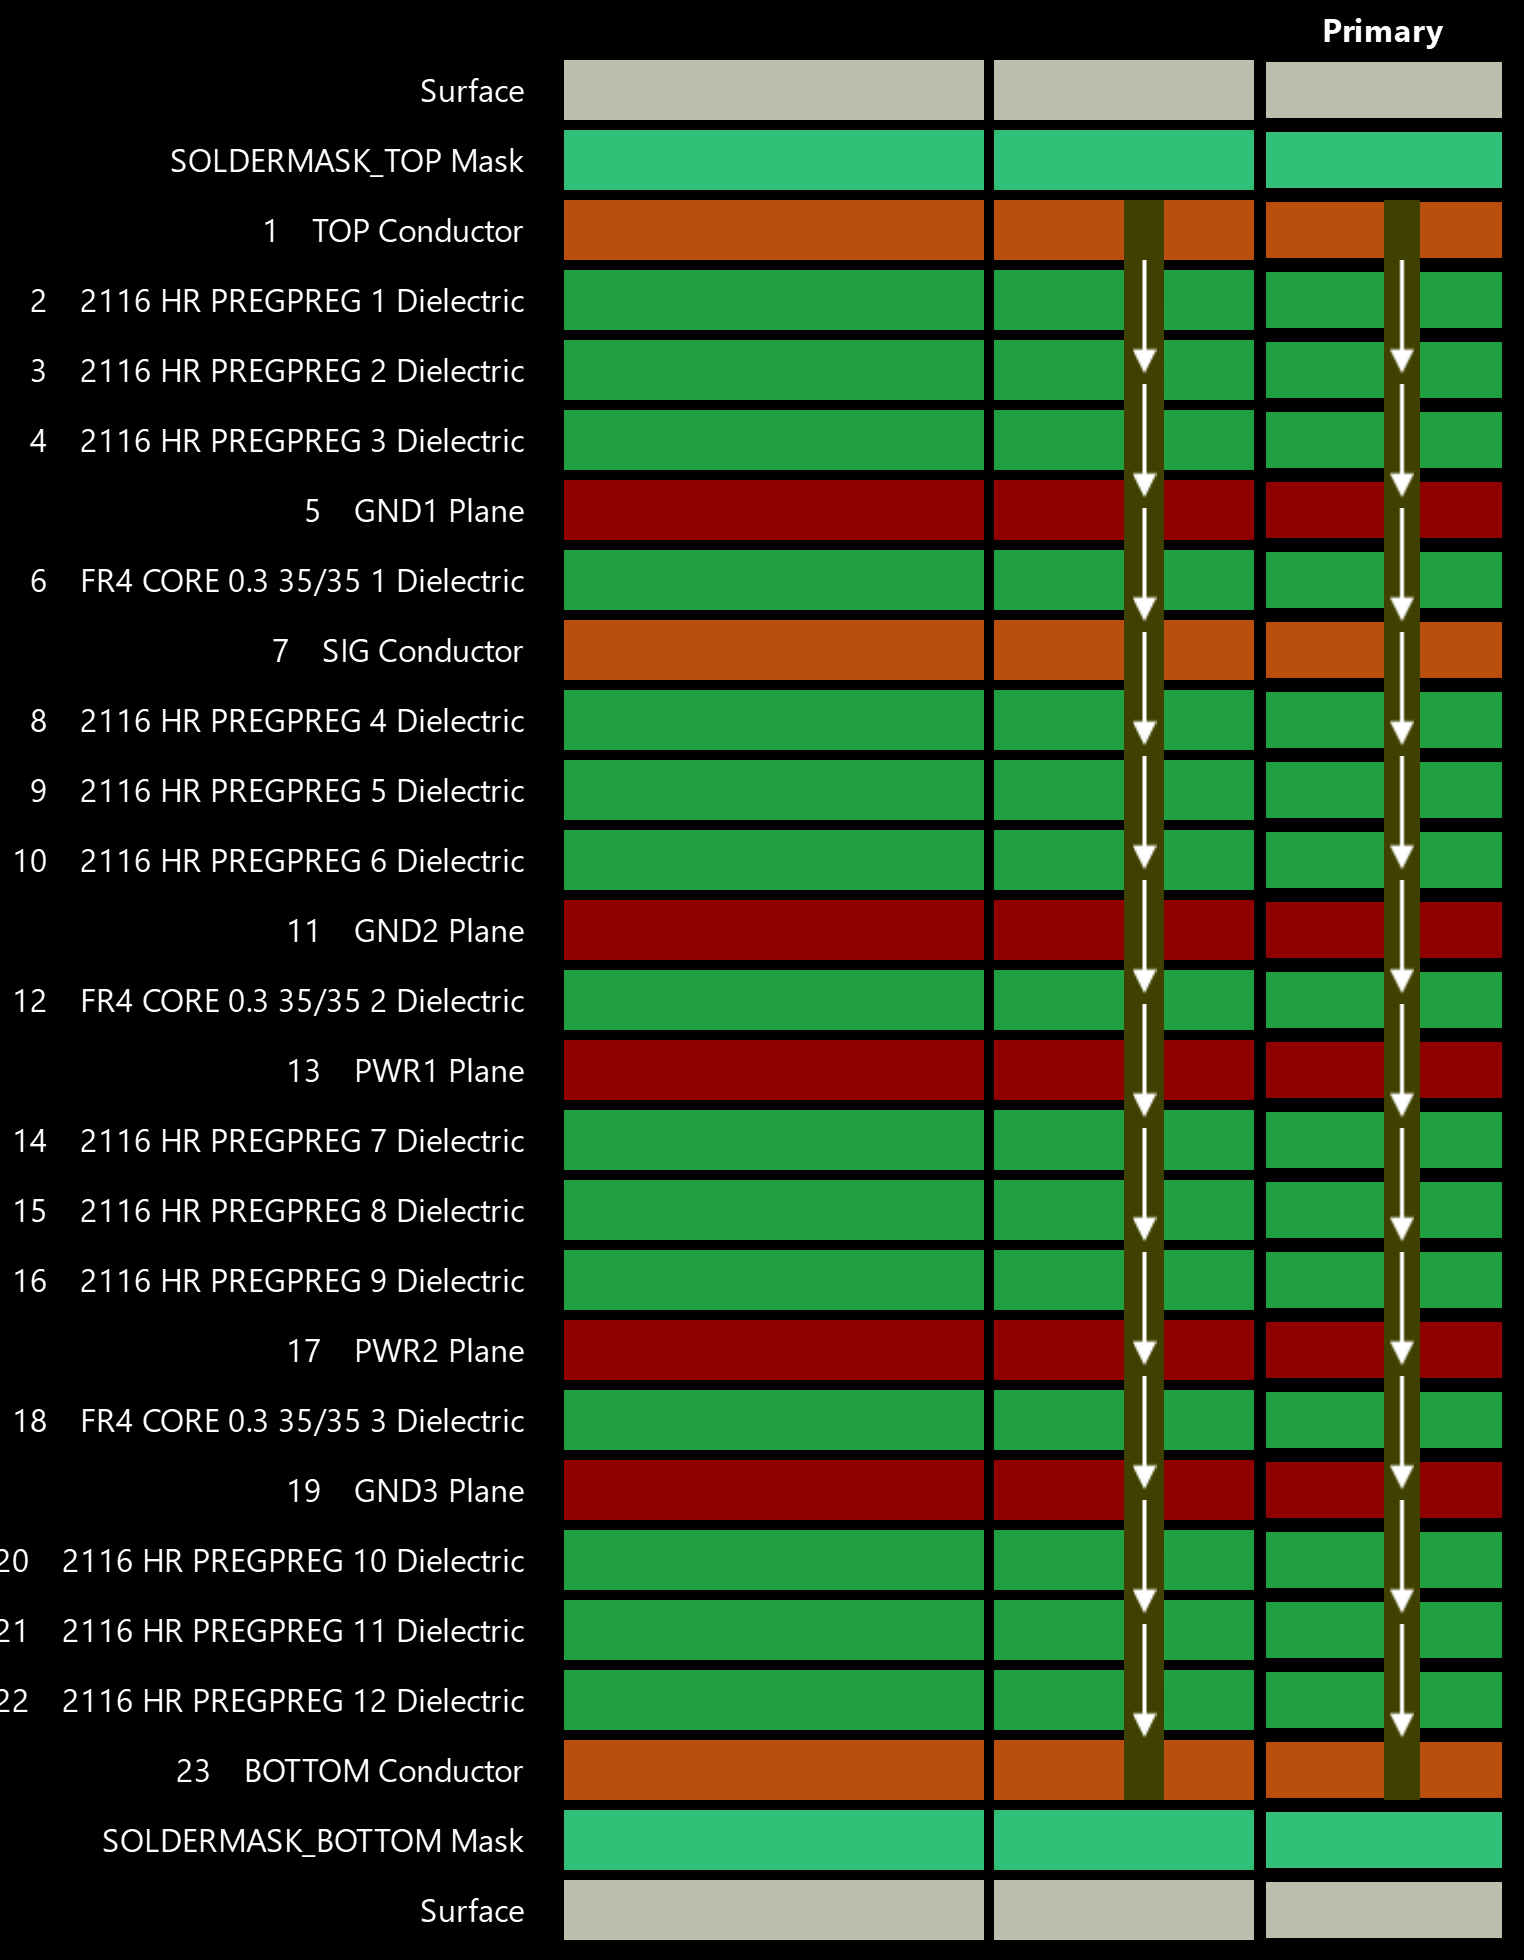
\includegraphics[width=0.8\linewidth]{gps_interface_board_ml_v97_cross_section_figure.png}
    \caption{Illustration of GIB main PCB cross-section}
    \label{fig:gib_main_pcb_cross_section_figure}
\end{figure}

\begin{figure}
    \centering
    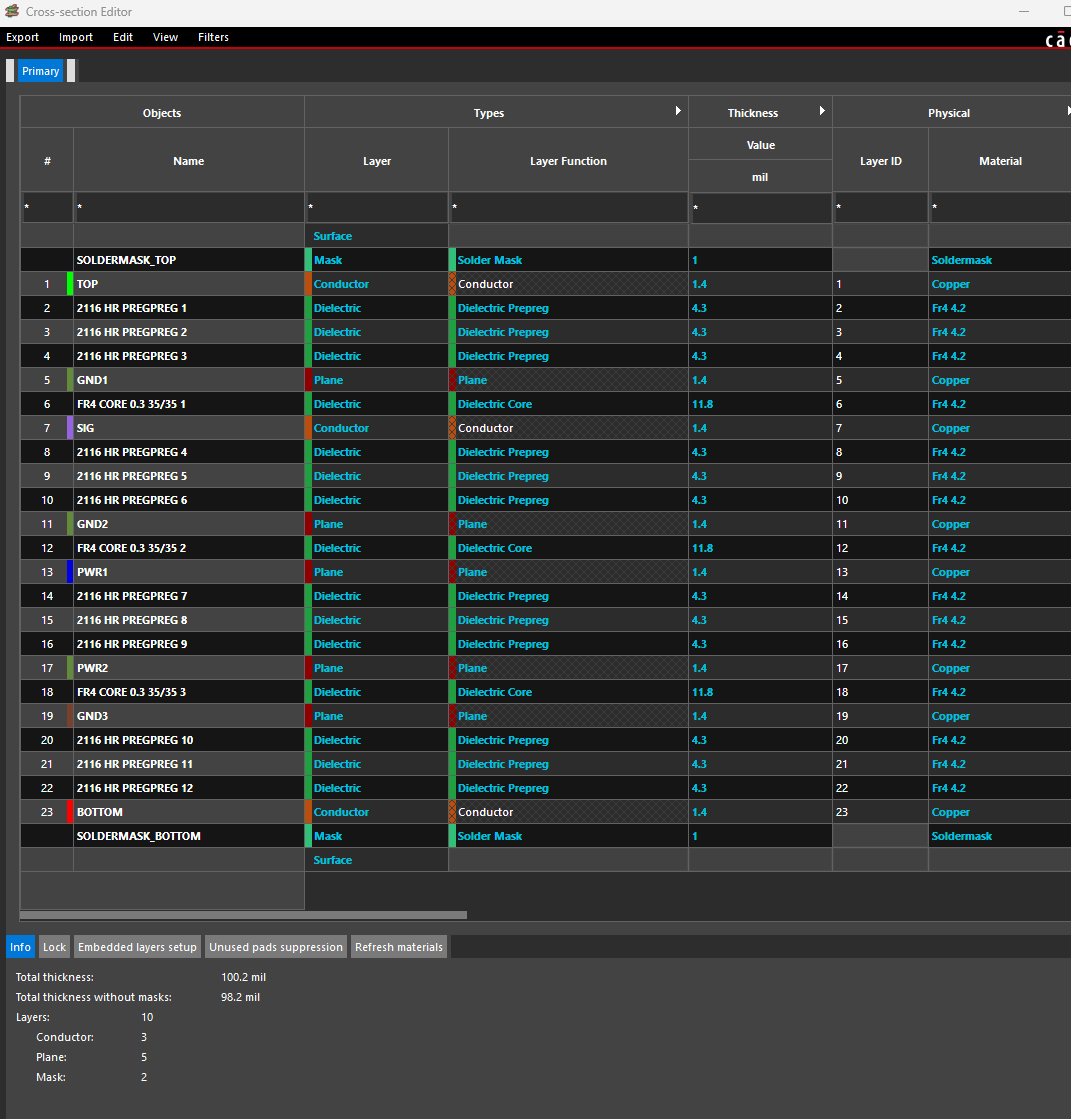
\includegraphics[width=0.8\linewidth]{gps_interface_board_ml_v97_cross_section_allegro_window.png}
    \caption{Details of GIB main PCB cross-section}
    \label{fig:gib_main_pcb_cross_section_details}
\end{figure}





A zip archive containing the manufacturing data for the GIB main PCB can be downloaded from \href{URL YYY}{EDMS xxxxx}

\section{Total Electrical Power}

Total electrical power of GIB - comprising of the main PCB, FPGA board, the slow control board and the fans is estimated to be at most 2 Amps at 12V. This is based on measurements from the current prototype 

\section{Optical Power}

Each DTS GIB will house up to six SFP optical transceivers. Each SFP will have a 1000Base-BX interface and a maximum laser power of 2mW at 1490,1550 or 1570nm. Because each individual SFP has an optical output power less than 5mW, and is hence a category 3R laser, no special safety precautions are needed.


%\section*{Acknowledgments}

\bibliographystyle{abbrv}
\bibliography{sample}

\end{document}